\documentclass[12pt]{beamer}
\usepackage[utf8]{inputenc}
\usepackage[portuguese]{babel}
\usepackage{graphicx}
\usepackage{colortbl}
\usepackage{color}
\usepackage{breqn}
\usepackage{listings}

\graphicspath{{./images/} {../images/}}

\definecolor{dkgreen}{rgb}{0,0.6,0}
\definecolor{gray}{rgb}{0.5,0.5,0.5}
\definecolor{mauve}{rgb}{0.58,0,0.82}
\definecolor{laranja_claro}{rgb}{1,0.9,0.5}
\definecolor{laranja_escuro}{rgb}{1,0.5,0.2}
\definecolor{azul_claro}{rgb}{0.5,0.9,1}

\lstset{frame=tb,
    language=C,
    frame=tb,
    aboveskip=3mm,
    belowskip=3mm,
    showstringspaces=false,
    columns=flexible,
    basicstyle={\small\ttfamily},
    numbers=left,
    numberstyle=\tiny\color{gray},
    keywordstyle=\color{blue},
    commentstyle=\color{dkgreen},
    stringstyle=\color{mauve},
    breaklines=true,
    breakatwhitespace=true,
    xleftmargin=.05\textwidth,
    xrightmargin=.05\textwidth,
    tabsize=4,
}

\definecolor{azul}{rgb}{0,0,.5}
\setbeamertemplate{navigation symbols}{}

\usetheme{Frankfurt}
\usecolortheme[named=azul]{structure}

%% Definindo o Autor e o título
\newcommand{\prof}{Newton Spolaôr}
\newcommand{\materia}{Compiladores}

\author[Grupo: c--]{Victor E. Almeida \and Marco A. G. Pedroso}

\title{Analisador léxico para a linguagem C- -}
\subtitle{Demonstrando o software}
\date{\today}
\institute{UNIOESTE}

\begin{document}
\frame{\titlepage}

\begin{frame}
\frametitle{Conteúdo}
\tableofcontents
\end{frame}

\section{Introdução}\label{Introdução}
\begin{frame}
    \frametitle{Softwares utilizados}
    \begin{itemize}
        \item \textbf{Sistema para compilar}: GNU make e gcc,
        \item \textbf{Linguagem de programação}: C11,
        \item \textbf{Gerador de analisador léxico}: GNU flex.
    \end{itemize}
\end{frame}

\section{lex/Flex}\label{lex/Flex}

\begin{frame}[t,fragile]{\insertsectionhead}
    \frametitle{Exemplo mínimo do flex}
    \begin{lstlisting}
        int num_lines = 0, num_chars = 0;

        %%
        \n      ++num_lines; ++num_chars;
        .       ++num_chars;
        %%

        int main() {
            yylex();
            printf("lines = %d, chars = %d\n",
                    num_lines, num_chars);
            return 0;
        }
    \end{lstlisting}
\end{frame}

\begin{frame}[t,fragile]{\insertsectionhead}
    \frametitle{Funcionamento do lex/flex}

    \begin{center}
        
    \begin{lstlisting}
    EXPRESSION_BEGIN "("
    {EXPRESSION_BEGIN} {
        doLog (
            LOG_TYPE_INFO,
            "inicio de expressao [(] encontrado"
        );
        is_open_expression++;
    }
    \end{lstlisting}
    \end{center}
    
\end{frame}

\section[Analisador]{Analisador léxico}\label{Analisádor léxico}
\begin{frame}[allowframebreaks]
    \frametitle{Lista de Tokens reconhecidos}
    \begin{itemize}
        \item\textbf{comando para o preprocessador}: ``\#''(.*)
        \item\textbf{palavras reservadas}: ``if''$|$``else''$|$``const''$|$``for''$|$``while''$|$``struct''
        \item\textbf{tipos de dados}:\\``int''$|$``float''$|$``double''$|$``char''
        \item\textbf{atribuição}: (``+''$|$``-''$|$``*''$|$``/''$|$``\%''$|$``$\ll$''$|$``$\gg$''$|$``\&''$|$``$|$''$|$``^'')$?$``$=$''
        \item\textbf{operador aritmético}:\\``+''``+''$?|$``-''``-''$?|$``/''$|$``*''$|$``sizeof''$|$\\``[''\{{\small INTEGER\_LITERAL}\}``]''
        \item\textbf{operador relacional}: ``\&\&''$|$``$||$''$|$``!''$|$(``=''$|$``!'')``=''$|$(``$<$''$|$``$>$'')``$=$''$?$
        \framebreak
        \item\textbf{fim de expressão}: ;
        \item\textbf{início de bloco}: \{
        \item\textbf{fim de bloco}: \}
        \item\textbf{abre parenteses}: (
        \item\textbf{fecha parenteses}: )
        \item\textbf{inteiro literal}: \{{\small DIGIT}\}+
        \item\textbf{float literal}: \{{\small INTEGER\_LITERAL}\}``.''\{{\small INTEGER\_LITERAL}\}
        \item\textbf{string literal}: \textbackslash{}``[\^{}\textbackslash{}\textbackslash{}\textbackslash{}n\textbackslash{}'']+
        \item\textbf{char literal}: \textbackslash{}`\textbackslash{}\textbackslash{}$?$.\textbackslash{}'
        \item\textbf{identificador}: (\{{\small LETTER}\})(\{{\small ALPHA\_NUM}\}$|$\_)*
    \end{itemize}
\end{frame}

\begin{frame}
    \frametitle{Mão na massa!!}
    \begin{figure}
        \centering
        
\includegraphics[width=.3\textwidth]{pizza.png}
        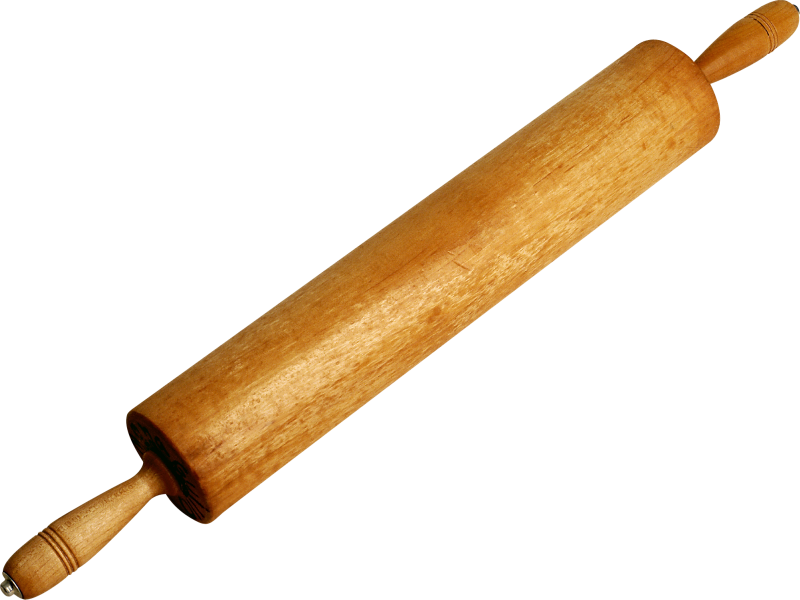
\includegraphics[width=.3\textwidth]{rolo.png}
        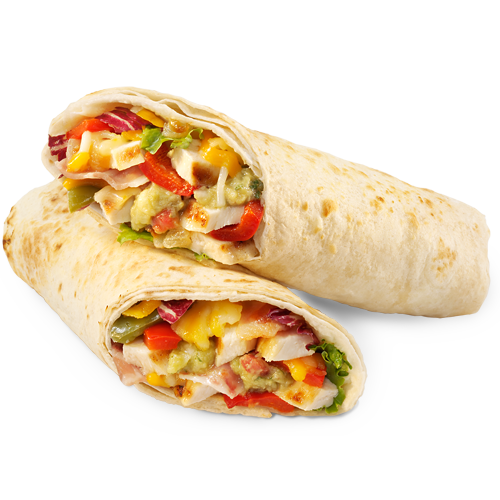
\includegraphics[width=.3\textwidth]{burrito.png}
    \end{figure}
\end{frame}

\section{Conclusão}
\begin{frame}
    \frametitle{Agradecimentos}
    \centering
    \Huge{Perguntas?}
    \begin{figure}
        \centering
        
\includegraphics[width=.3\textwidth]{alerta.png}
        
\includegraphics[width=.3\textwidth]{perigo.png}
        
\includegraphics[width=.3\textwidth]{eletricidade.png}
    \end{figure}
    \Huge{Obrigado pela atenção}
\end{frame}

\end{document}
